\documentclass[letterpaper, 10pt]{book}

\newcommand{\version}{%%%VERSION%%% }
\newcommand{\url}[1]{\texttt{#1}}

\title{QSim Version \version User Guide}
\author{Chad D. Kersey\\ Georgia Institute of Technology\\ Atlanta, GA 30332}

\usepackage{verbatim}
\usepackage{graphicx}
\usepackage[right=1.5in, top=1in, bottom=1in, left=1.0in]{geometry}
%\oddsidemargin=0.5in

\begin{document}
\maketitle

\setcounter{tocdepth}{1}
\tableofcontents

\chapter*{Introduction}
QSim is a thread safe multicore emulation library based on the QEMU emulator.
QSim provides instruction-level control of the emulated environment and 
detailed information about the executing instruction stream. X86 Linux guests
are supported with hundreds of emulated hardware contexts, each of which can run
in an independent host thread. Applications of QSim include trace-gathering,
multithreaded software development, and its primary target: microarchitecture
simulation.

In the domain of microarchtiecture simulators, the advantage of using a library
like QSim is that the instruction set is emulated with high fidelity by QEMU, so
the simulator only needs to implement those aspects of the instruction set
relevant to its results. This has both advantages and disadvantages that have
been discussed at length elsewhere.

%%% TODO: Filler text about how great simulation is or somesuch? This section 
%%%       looks fairly thin at 2 paragraphs.

\section{Requirements}
The following are needed to run QSim on your machine. Before you attempt to build and run QSim, make sure these are available:

\begin{itemize}
  \item{64-bit CPU and operating system}
  \item{2GB of RAM and at least 4GB of swap}
  \item{Libraries and compiler to build 32-bit binaries}
\end{itemize}

\chapter{QSim Software Architecture} \label{chap:arch}
QSim is an effort in combining several large and complex open source software
packages into a single entity. The QSim code is very small compared to the
QEMU and Linux codebases it leverages. These other projects are not included
with QSim, but are downloaded and patched by the provided scripts
\texttt{getqemu.sh} and \texttt{getkernel.sh}.

\section{QSim Design}

\subsection{The QEMU Emulator}

\begin{figure}
\begin{center}
\includegraphics[width=3in]{qemu_diagram}
\caption{Block diagram of QEMU.}
\label{fig:qemu}
\end{center}
\end{figure}

A block diagram of QEMU is shown in Figure~\ref{fig:qemu}. QEMU is an open
source PC emulator that uses dynamic binary translation to translate guest
instructions to a host instructions in the translation cache. Multiple
guest architectures are supported, both as guests and hosts, including x86,
SPARC, and PowerPC. The environment provided by QSim allows an operating system
and applications to be run in an emulated environment, instruction by
instruction, on multiple emulated cores. Currently only 32-bit x86 guests are
supported, but other architectures are expected to become available.

\begin{figure}
\begin{center}
\includegraphics[width=5in]{translation}
\caption{QEMU translation process with expansion of return instruction from a
  guest basic block.}
\label{fig:translation}
\end{center}
\end{figure}

Figure~\ref{fig:translation} illustrates the QEMU translation process. This is a
two-step process in which guest instructions are translated into Tiny Code
Generator (TCG) operations and then host instructions. QSim allows the creation
of \emph{helper functions}, which are functions that can be called from the
translation cache. QEMU uses helper functions to implement uncommon but complex
guest instructions, so that they do not have to be implemented entirely as large
and complex blocks of code that are compiled at run-time.

QSim uses the helper function mechanism to instrument guest instructions. Calls
to helper functions are added to the translations of instrumented instructions.
From these helper functions, callbacks that have been registered by the user's
program are called.

\subsection{The QSim Library}

\begin{figure}
\begin{center}
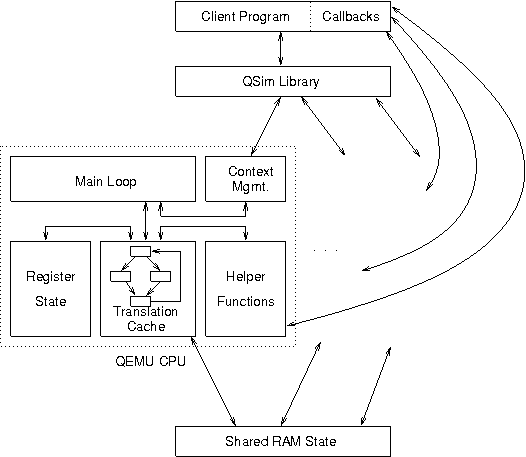
\includegraphics[width=4in]{qsim_diagram}
\caption{Block diagram of QSim library design with arrows representing data flow
         between components.}
\label{fig:qsim}
\end{center}
\end{figure}

Figure~\ref{fig:qsim} is an illustration of the fully-integrated QSim software
architecture. The QEMU emulator, as seen in Figure~\ref{fig:qemu} is present,
replicated once per simulated hardware context and sharing guest RAM state. The
QSim library makes calls into these QEMU CPUs on behalf of the client program,
and the QEMU CPUs make the callbacks into the client programs based on events in
the instruction stream. A variety of different callbacks are provided,
including:

\begin{itemize}
  \item{Every instruction}
  \item{Atomic memory operations}
  \item{Memory reads/writes}
  \item{Register reads/writes}
  \item{Interrupts}
  \item{``Magic'' CPUID instructions}
\end{itemize}

The atomic memory operation and read/write callbacks are given in addition to
the instruction callbacks for their corresponding instructions. Magic
instructions are used to provide out-of-band communication between the guest and
QSim, and are explained in detail in Section~\ref{sec:magic}.

\subsection{Guest Environment}

The QSim guest environment includes the Linux kernel, the Busybox all-in-one
userland, an init script, and a statically-linked application binary. Since QSim
currently provides no emulation of disk or network devices, guest programs are
loaded as part of a Linux inital RAM filesystem.

Porting applications to the guest environment and building the Linux kernel
image is discussed at length in Chapter~\ref{chap:porting}.

\subsection{Remote QSim}

For environments where detailed, distributed high-core-count simulations are
performed, QSim provides a client/server version that can operate over a
network. Each server is intended to support hundreds of clients, one for each
simulated hardware context. Further discussion of remote QSim is in
Chapter~\ref{chap:remote}.


\subsection{QDB, The QSim Debugger}

QDB provides a commandline interface to QSim that can be used to debug guest
applications, geust operating systems, and the QSim library itself. Compared to
the rest of QSim, QDB is in an earlier state of development. It is for this
reason that QDB maintains its own list of bugs and unimplemented features.

\subsection{The Fastforwarder}\label{sec:fastforwarder}
\begin{figure}
\begin{centering}
\includegraphics[width=4in]{fast_forwarder}
\caption{Operation of \texttt{qsim-fastforward} generates a reuseable state
         file.}
\label{fig:fastforwarder}
\end{centering}
\end{figure}

The QSim fastforwarder, \texttt{qsim-fastforward} is used to generate state
files that represent the state of RAM after the machine has booted, but before
the application has began running. This is so that the potentially very
long time spent waiting for Linux to boot can be amortized over all simulations
using a given \texttt{bzImage} and number of QEMU CPUs.

\section{QSim Directory Hierarchy}
What follows is a tour of the directory structure of the QSim codebase. This is
provided as both a reference and an introduction.

\subsection{Documentation}

\begin{verbatim}
    INSTALL
    README
    doc/
    doc/web
\end{verbatim}
\texttt{doc/} contains this document, of which \texttt{README} is an abridged
version. \texttt{INSTALL} is a simple runlog containing all of the commands
needed to create a useable QSim installation.

\texttt{doc/web} is the QSim website, included here so that it may be modified
under version control as needed.

\subsection{QSim Core}

\begin{verbatim}
    qsim.h
    qsim-regs.h
    qsim-vm.h
    qsim-context.h
    mgzd.h
    vm-func.h
    qsim.cpp
    Makefile
\end{verbatim}
These files form the core of QSim. \texttt{qsim-regs.h} defines 
\texttt{enum regs}, an important enumeration of guest register names shared
between the modifications to QEMU and QSim. \texttt{qsim-vm.h} defines the
types of the basic callback functions that are called from within QEMU, as well
as \texttt{qemu\_ramdesc\_t}, a structure used to describe guest RAM areas
within QEMU to allow sharing of memory between multiple instances of QEMU.
\texttt{mgzd.h} and \texttt{qsim-context.h} provide the services necessary to
maintain multiple separate instances of QEMU as though they were components of
the same program. \texttt{qsim.h} and \texttt{qsim.cpp} are the actual nuts
and bolts of QSim. \texttt{qsim.h} must be included by any client program
of QSim and \texttt{qsim.cpp} is the only source in what becomes
\texttt{qsim.so}.

\texttt{Makefile} leaves a lot to be desired, but it is responsible for
building QSim. For more information on building QSim, see \texttt{INSTALL} in
the QSim root directory. 

\subsection{Fast Forwarder}
\begin{verbatim}
    fastforwarder.cpp
    statesaver.cpp
    statesaver.h
\end{verbatim}
These files ocmpile to a program called \texttt{qsim-fastforwarder}, which is 
used as described in Section \ref{sec:fastforwarder} to eliminate the start-up
portion of long simulations, especially ones with high core counts.

\subsection{QEMU}
\begin{verbatim}
    getqemu.sh
    qemu-0.12.3.qsim.patch
    qemu-0.12.3/
\end{verbatim}
This directory appears after \texttt{getqemu.sh} has been run and contains the
modified QEMU. The result of a successful compile of QEMU for QSim is a shared
object file which will be used by the QSim library.

\subsection{Initial Ram Filesystem}
\begin{verbatim}
    initrd/
    initrd/init
    initrd/mark_app.c
    initrd/qsim_io.c
    initrd/test_threads.c
    initrd/busybox-1.16.1
    initrd/etc
\end{verbatim}
The \texttt{initrd} directory contains the userspace portion of the guest
environment, which is packaged into a Linux initial RAM filesystem and compiled
into the Linux kernel. Information on how to configure the guest system is in
Chapter~\ref{chap:porting}.

\subsection{Linux Kernel Sources}
\begin{verbatim}
    linux/
    linux/getkernel.sh
    linux/linux-2.6.34.qsim.patch
    linux/bzImage
    linux/linux-2.6.34/
\end{verbatim}
A modified Linux kernel is used by QSim. The \texttt{getkernel.sh} script
downloads the unomdified kernel from upstream and patches it with modifications
that allow it to boot in QSim guest environment, without using BIOS or usual PC
hardware services that QSim does not provide.

\subsection{Disassembler}
\begin{verbatim}
    distorm/
\end{verbatim}
Several of the examples and the QSim Debugger require a disassembler. Distorm 
was chosen as a simple, portable, open source disassembly library. Note that it
is not part of QSim proper; it is just a utility library that the bundled
applications happen to require that was considered uncommon enough to be
included with the source distribution.

\subsection{Remote QSim}
\begin{verbatim}
    remote/
    remote/README
    remote/qsim-net.h

    remote/client
    remote/client/Makefile
    remote/client/qsim-client.cpp
    remote/client/qsim-client.h
    remote/client/client.cpp

    remote/server
    remote/server/Makefile
    remote/server/server.cpp
\end{verbatim}

Remote QSim, covered in detail in Chapter~\ref{chap:remote}, is a simple way to
share a single instance of the QSim emulator among several remote processes.
Remote QSim includes a server program (\texttt{server.cpp}), the client library
(\texttt{qsim-client.h}, \texttt{qsim-client.cpp}), and a sample remote client
program (\texttt{client.cpp}).

\subsection{Simplesim}
\begin{verbatim}
    simplesim/
\end{verbatim}
SimpleSim is an example multicore out-of-order CPU simulator.
%TODO: Expand this section!

\subsection{Examples}
\begin{verbatim}
    examples/
    examples/qtm.cpp
    examples/simple.cpp
    examples/io-test.cpp
    examples/vistrace.cpp
\end{verbatim}
The ``examples'' are example client program using the QSim library. One of
these, \texttt{simple.cpp}, is examined in detail in Chapter~\ref{chap:example} 
as an example client program using QSim.

\subsection{QDB: The QSim Debugger}
\begin{verbatim}
    qdb/
    qdb/BUGS
\end{verbatim}
QDB provides a commandline interface to a QSim, running one guest CPU per host
thread. QDB allows users to load in symbol tables for both the kernel and
individual user address spaces. It also provides dynamic instruction count
based flat profiling with uniform statistical sampling. The best documentation
for QDB is its own built-in help system, which can be accessed at any time by
typing \texttt{help}.

\section{Magic Instructions} \label{sec:magic}

\begin{table}
\begin{tabular}{c|l}
  \textbf{Value in \texttt{\%rax}}&\textbf{Function}\\
  \texttt{0xc501e0xx}&Console output, character \texttt{x}.\\
  \texttt{0x1d1e1d1e}&Calling CPU now executing idle loop.\\
  \texttt{0xc75cxxxx}&Context switch to TID \texttt{x}.\\
  \texttt{0xb007xxxx}&Bootstrap CPU \texttt{x}, \texttt{\%ip} provided by
                      subsequent magic instruction.\\
  \texttt{0x1dxxxxyy}&Inter-processor interrupt. Interrupt CPU \texttt{x} with
                      vector \texttt{y}.\\
  \texttt{0xc7c7c7c7}&Request CPU count, returned in \texttt{\%rax}.\\
  \texttt{0x512e512e}&Request RAM size in MB, returned in \texttt{\%rax}.\\
  \texttt{0xaaaaaaaa}&Application start signal. Causes application start 
                      callback to be called.\\
  \texttt{0xfa11dead}&Application end signal. Causes application end callback
                      to be called.\\
\end{tabular}
\caption{Magic Instructions provided by \texttt{OSDomain}.}
\label{table:magic}
\end{table}

QSim provides an interface for out-of-band communication between the guest
environment, QSim library, and its client programs, through use of magic
instructions. Magic instructions are QSim-defined regions of the CPUID address
space that perform special functions. CPUID is ordinarily used by software to
get information about the CPU on which it is running. A value is loaded into RAX
and once the CPUID instruction has run, the registers are set according to the
results. This is used ordinarily to query CPUs for features.

In QSim, the magic instructions are used to provide simplified, paravirtualized,
emulated hardware. Magic instruction callbacks can also be set by client
programs to extend this interface. Table~\ref{table:magic} lists the magic
instructions defined by QSim itself and used by the Linux kernel and some of the
guest software.

\chapter{Remote QSim} \label{chap:remote}

\begin{figure}
\begin{centering}
\includegraphics[width=6in]{remote_diagram}
\caption{Remote QSim allows multiple clients to connect to a QSim server.}
\label{fig:remote}
\end{centering}
\end{figure}

QSim, in addition to providing a local library, also provides a remote version
that can be used over a network. This is to allow the use of QSim in
distributed architectural simulations where the front end emulation is not
considered a bottleneck.

Figure~\ref{fig:remote} is a block diagram of the QSim remote architecture. The
server is an ordinary client program to an instance of the local QSim library.
Remote clients connect over the network using the QSim Client library, which
provides an interface very similar to the local \texttt{OSDomain} to the remote
clients.

\section{Using the Server}

The QSim server is in \texttt{remote/server} and can be built by running
\texttt{make} in that directory. Once built, running the server with no command
line options will display its usage. It takes the following command line options
in the given order:

\begin{itemize}
  \item{The port to listen for incoming to connections on}
  \item{Number of QEMU CPUs (simulated hardware contexts)}
  \item{Path to kernel image file}
  \item{Optional size of guest RAM in megabytes}
\end{itemize}

An example is:

\begin{verbatim}
    $ ./server 1234 2 bzImage
\end{verbatim}

The QSim server sends console output to the console on which it is started, so
expect the usual boot messages. To test this server, the sample client can be
started with:

\begin{verbatim}
    $ ./client localhost 1234
\end{verbatim}

This is also the port address used by the simple example program covered in
Chapter~\ref{chap:example}, the remote version of which is built as 
\texttt{examples/simple-client}.

\section{Writing a Client}

A remote QSim client differs from an ordinary QSim client program primarily in
using \texttt{Qsim::Client} instead of the usual \texttt{Qsim::OSDomain}. Many
of the API calls are similar. The program listed in Chapter~\label{chap:example}
is a great example of the differences.

\chapter{A Sample Client Program} \label{chap:example}
The use of QSim fundamentally boils down to a few simple steps that a client
program must take:
\begin{itemize}
  \item{Instantiate one (and only one) \texttt{OSDomain}.}
  \item{Attach instrumentation to that \texttt{OSDomain}.}
  \item{Call \texttt{run()} on that \texttt{OSDomain}, ocasionally calling
        \texttt{timer\_interrupt()}.} 
  \item{Do something with the information collected by the instrumentations.}
\end{itemize}

The last step is purely optional, but there would not be much reason to use
QSim without the instrumentation.

For the purposes of this Chapter, we will examine \texttt{examples/simple.cpp},
the simple example; a multicore trace gathering utility.

\section{Operation}

\begin{figure}
\begin{center}
\includegraphics[width=5in]{simple_example}
\caption{Design of the \texttt{simple.cpp} example program.}
\label{fig:simplecpp}
\end{center}
\end{figure}

As illustrated in Figure~\ref{fig:simplecpp}, \texttt{simple.cpp} is basically a
trace gatherer. It installs a set of callbacks that print messages to a textual
trace file whenever they are called.

\section{Listing}
\verbatiminput{simple.cpp.num}

\section{Instantiating \texttt{OSDomain}}
As is often found in simple QSim client programs, the single \texttt{OSDomain}
(there can only be one) is allocated on the heap in the \texttt{main()}
function at lines 123 through 132. This allows the same \texttt{osd} reference
to be used for either an \texttt{OSDomain} constructed with a number of CPUs and
a kernel image or an \texttt{OSDomain} constructed from a state file.

If the \texttt{QSIM\_REMOTE} macro is defined, this will not be done, and
instead a \texttt{Qsim::Client} will be created, connecting to a predefined
host and port.

\section{The Callback System}

\texttt{simple.cpp} uses instruction, atomic, memory, interrupt, and I/O
callbacks and logs the occurrence of each to a trace file. Application start
and end callbacks are used. \texttt{TraceWriter::app\_start\_cb()} sets the
callbacks that perform tracing, and \texttt{TraceWriter::app\_end\_cb()}
sets a flag that causes the main loop to exit.

\texttt{app\_start\_cb()} is not called in remote QSim. Instead, fast-forwarding
to the application start is done automatically, before any clients are allowed
to connect. If \texttt{QSIM\_REMOTE} is set, the application start callback is
called by the \texttt{TraceWriter} constructor instead, and no start or end
callbacks are set.

\chapter{Porting Guest Software} \label{chap:porting}
Currently, there are two available methods for loading guest software into QSim.
It can be compiled into the kernel image, or it can be transferred to the guest
environment through the \texttt{initrd/qsim\_io.c} program. With the former 
method, the mechanism through which they are loaded is the Linux initial RAM f
ilesystem (\texttt{initramfs}). This allows a root filesystem to be included
along with the kernel image and mounted at start-up, even without support for
disks.

The latter method involves using the \texttt{initramfs} and the
\texttt{qsim\_io} program to transfer a program. The default \texttt{init}
script does this. An example of a client program that transfers a file in this
manner is in \texttt{examples/test-io.cpp}.

Porting an application to QSim consists of the following steps:

\begin{itemize}
  \item{Compile the application for 32-bit Linux, statically linked.}
  \item{Copy the application and all needed files into \texttt{initrd/sbin}.}
  \item{Modify the \texttt{initrd/init} script appropriately.}
  \item{Run \texttt{make} in \texttt{initrd} to build \texttt{initrd.cpio}.}
  \item{Run \texttt{ARCH=i386 make} in the Linux kernel root to create 
        \texttt{bzImage}, the kernel image which will be loaded into the QSim
        address space.}
\end{itemize}

\section{Compiling for QSim}
On a 64-bit host, creating 32-bit statically-linked binaries is a matter of 
passing the \texttt{-m32} option to the GCC compiler and the \texttt{-static}
option to the linker. In a typical GNU Autotools based build environment, this
can be accomplished with:

\begin{verbatim}
    $ CFLAGS=-m32 CXXFLAGS=-m32 LDFLAGS=-static ./configure
    $ make
\end{verbatim}

The \texttt{file} command can be used to ensure that the resulting binary is
actually a 32-bit statically-linked ELF.

\section{Setting Up the Linux Initial Ramdisk}
The \texttt{initrd} makefile is set up so that any files placed in 
\texttt{initrd/sbin} will be added to the generated \texttt{initrd.cpio}. User
applications are not, however, included as dependencies, so when modifying them
it is prudent to perform a \texttt{make clean} before running \texttt{make} to
produce the ramdisk file. Typically the only actions required to set up the
linux filesystem is to copy the application binary into \texttt{initrd/sbin},
modify the \texttt{initrd/init} script to launch the application, and run
\texttt{make clean} followed by \texttt{make}.

The \texttt{init} script contains, out of the box, a set of sample application
invocations commented out with octothorpes. If using one of the prepackaged
benchmarks, it is only necessary to uncomment the corresponding line. 
Otherwise, the appropriate command can be added anywhere between the invocation
of \texttt{mark\_app} and \texttt{mark\_app END}.

\subsection{Busybox Utility Programs}
The command interpreter used to execute the \texttt{init} script, as well as
most of the utility programs available within it (\texttt{cat}, \texttt{grep},
\texttt{ls}) are provided by the Busybox all-in-one userland.
It provides smaller-footprint versions of common Unix utilities, accessed by a
set of symbolic links to the same file.

\subsection{QSim Guest Utilities}
The initial ramdisk also contains a set of QSim-specific utilities and test
programs:

\begin{verbatim}
    qsim-out
\end{verbatim}
Uses the magic instruction mechanism to copy program input to the QSim console.

\begin{verbatim}
    mark_app [END]
\end{verbatim}
Uses the magic instruction mechanism to mark the start and end of the
application. This causes the application start and end callbacks described on
pages \pageref{func:set_app_start_cb}-\pageref{tf:set_app_end_cb} to be called.


\begin{verbatim}
    test-threads
\end{verbatim}
Simply spawns 100 threads and waits for them to exit. Each thread grabs a
mutex, prints a message, and exits. Used to check that atomic memory operations
are being treated as such by the client program; not a simple task if this
application is multithreaded.

\section{Compiling the Kernel Image}

Initially, the kernel image must be configured with the absolute path to the
\texttt{initrd.cpio} file. The configuration system can be launched by changing
to the kernel root and running:

\begin{verbatim}
    $ ARCH=i386 make menuconfig
\end{verbatim}

The option to configure the path to the RAM disk CPIO file is under ``General
Options''. After this initial configuration has been performed, subsuquent
builds only require the second step of the process, running \texttt{make} with
\texttt{ARCH} set to \texttt{i386}:

\begin{verbatim}
    $ ARCH=i386 make
\end{verbatim}

\section{Using the Kernel with QSim}
A symlink to the kernel this produces is conveniently placed in the
\texttt{linux/} directory. This is the default kernel image as used by all of
the programs in \texttt{examples/}. QDB takes the path of the kernel image as a
commandline option. Within client programs, the path to the kernel is an
argument to the \texttt{OSDomain} constructor (see \texttt{OSDomain}, page 
\pageref{class:OSDomain} for details).

\chapter*{Glossary}

\begin{description}
\item[atomic memory operation]
A memory operation that is required by the architecture to complete as an
indivisible operation. Atomic read-modify-write operations like \texttt{XCHG} 
are used in the implementation of synchronization primitives.

\item[callback]
A function passed as an argument to another layer of the software stack, so
that it can be called by software in that layer as necessary. In QSim, 
callbacks are code within the \emph{client program} that is called from
\emph{helper functions}. Callbacks are the primary way QSim allows its users to
instrument the code executing in the \emph{guest}. The word ``callback'' can
also be used to refer to the instance of a specific call to a callback
function. For example, ``A memory operation callback will be received after any
exception conditions on the address being accessed are cleared up.'' In this 
sentence, the ``memory operation callback'' is not the function itself, but a 
specific instance of a call to the function.

\item[client program]
An application that makes use of a library; for the purposes of this document
the ``client program'' is always an application that uses QSim.

\item[guest]
The simulated system, or virtual machine, within QSim. Often used as an
adjective to describe a data structure: ``guest CPU state;'' the registers of 
the virtual CPU stored in a data structure within QEMU, ``guest RAM;'' the 
memory image of the guest machine. Used as an antonym of \emph{host}, the
machine on which QSim and the client program runs.

\item[helper function]
Part of QEMU, a C function intended to be called from the 
\emph{translation cache}. Helper functions are used to implement \emph{guest}
functionality that is complex and not time critical. Their use results in more
compact translated code and a simpler binary translator.

\item[host]
The machine on which QSim and its client program runs, antonym of 
\emph{guest}. Used to describe abstractions that may otherwise be confused for
aspects of the guest system: ``host virtual address'',
``host instruction set.''

\item[magic instruction]
An instruction that provides a service not found in current hardware,
decoded using an unorthodox mechanism. In QSim, magic instructions are
\texttt{CPUID} instructions initiated with invalid values in \texttt{\%rax}.
These can be tied to callbacks and used to implement new features or create
debugging output.

\item[OS domain]
A collection of CPUs among which memory is sequentially consistent and cache
coherent, usually associated with a single operating system image. The 
\texttt{OSDomain} class gets its moniker from this concept.

\item[QEMU CPU]
A hardware context within QEMU. Not to be confused with a CPU in the sense
of an entire chip, or in the sense of a core within that chip that may 
support multiple contexts through and SMT arrangement. A four-core chip with
2-way SMT, for example, would be emulated with 8 QEMU CPUs.

\item[remote QSim]
The distributed version of the QSim library. Separates functionality into an
emulation server and a client which exports an API similar to locally-running
QSim.

\item[translation cache] 
The data structure into which a dynamic binary translator like QEMU places the
result of translation and from which the translated code is run. The only
code emulating \emph{guest} instructions is executed by the \emph{host}
through the translation cache, either directly or by calling 
\emph{helper functions}.
\end{description}

%%%%%%%%%%%%%%%%%%%%%%% End Main Text; Begin Appendices %%%%%%%%%%%%%%%%%%%%%%%
\appendix
\chapter{API Documentation}

What follow are descriptions of the user-facing classes of which QSim is 
comprised and their interfaces, member types, and member variables. By far
the most important class of these is \texttt{OSDomain}, as described in
Chapter~\ref{chap:example} and documented on page \pageref{class:OSDomain}.
Entire simulators can be built interacting only with \texttt{OSDomain}. The
other available classes provide various utility functions and the ability to
interact directly with the QEMU CPU objects that normally comprise an
\texttt{OSDomain}.

The most important utility class is \texttt{Queue}, described on page
\pageref{class:Queue}. It provides a way to delay the processing of execution
events until after they have been emulated. Use of Queues allows all of the
processing of events to be centralized within a single main loop instead of
scattered through multiple callbacks. Although this results in a loss of control
over the instruction-level timing in QSim, it is ideally suited for applications
in which this is irrelevant or of diminished importance, such as trace
generation and simple application evaluation.
\newpage

\section{\texttt{Qsim::OSDomain}} \label{class:OSDomain}

\texttt{OSDomain} is a singleton class that creates and manages a multicore
processor emulator. The simplest way to use QSim is to instantiate a QSim
\texttt{OSDomain}, provide it with a set of callbacks or a \texttt{Queue}, and
start running instructions on it, periodically calling 
\texttt{OSDomain::timer\_interrupt()}. This is exactly what the sample program
in Chapter \ref{chap:example} does. \texttt{OSDomain} means ``Operating System
domain.'' It is so named because all of the CPUs in it share one cache coherent
and sequentially consistent block of RAM that contains a single OS image.

\subsection{Member Types}
\label{enum:cpu_mode} \begin{verbatim}
    enum cpu_mode {
      MODE_REAL, MODE_PROT, MODE_LONG
    };
\end{verbatim}

Used to describe the current mode of the CPU. While 32-bit real mode and 16-bit
protected mode do exist on the hardware, for modern operating systems it can be
assumed that \texttt{MODE\_REAL} means 16-bit default operand sizes and is only
encountered during boot, and \texttt{MODE\_PROT} means 32-bit default operand
sizes. \texttt{MODE\_LONG} only works in protected mode, and has 64-bit default
operand sizes.

\label{enum:cpu_prot} \begin{verbatim}
    enum cpu_prot {
      PROT_KERN, PROT_USER
    };
\end{verbatim}

Describes the current protection level of the CPU. While x86 actually provides
a MULTICS-like ring system complete with hardware-defined task and call gate
structures and four levels of protection, these still exist only for backwards
compatability. This data type is used to describe whether a given CPU within
QSim is running in supervisor mode (ring 0) or user mode.

\subsection{Member Functions}
\label{func:OSDomain} \begin{verbatim}
    OSDomain(uint16_t    n, 
             std::string kernel_path, 
             unsigned    ram_mb = 2048);
\end{verbatim}

This \texttt{OSDomain} constructor takes as parameters \texttt{n}, the number of
CPUs, \texttt{kernel\_path}, the path to an appropriate \emph{bzImage} and 
optionally \texttt{ram\_mb}, the size of system RAM in megabytes. 

\begin{verbatim}
    OSDomain(const char *state_file);
\end{verbatim}

The other \texttt{OSDomain} constructor loads the state from a file. This allows
for fast startup compared to emulating the entire boot process.

\label{func:idle} \begin{verbatim}
    bool idle(unsigned i);
\end{verbatim}

Returns true if CPU \texttt{i} is running its idle loop according to the OS,
false otherwise.

\label{func:get_tid} \begin{verbatim}
    int get_tid(uint16_t i);
\end{verbatim}

If Linux has booted, returns the task ID of the thread currently running on CPU
\texttt{i}. Otherwise returns $-1$.

\label{func:get_mode} \begin{verbatim}
    enum cpu_mode get_mode(uint16_t i);
\end{verbatim}
Returns the mode (real, protected, or long) of CPU \texttt{i} (see 
\texttt{enum cpu\_mode}, page \pageref{enum:cpu_mode}). Not capable of 
distinguishing 16-bit protected mode, but this is not used by any current OS.

\label{func:get_proc} \begin{verbatim}
    enum cpu_prot get_prot(uint16_t i);
\end{verbatim}
Returns the current protection ring (kernel or user) of CPU \texttt{i} (see
\texttt{enum cpu\_prot}, page \pageref{enum:cpu_prot}).

\label{func:get_n} \begin{verbatim}
    int get_n() const;
\end{verbatim}
Returns the number of CPUs being emulated.

\label{func:get_ramdesc} \begin{verbatim}
    qemu_ramdesc_t get_ramdesc() const;
\end{verbatim}
Returns the \texttt{qemu\_ramdesc\_t} structure used by the instances of QEMU
within this \texttt{OSDomain} to share their memory region (see 
\texttt{qemu\_ramdesc\_t}, page \pageref{struct:qemu_ramdesc_t}).

\label{func:run} \begin{verbatim}
    unsigned run(uint16_t i, unsigned n);
\end{verbatim}
Run the emulator on CPU \texttt{i} for \texttt{n} instructions or until an
exception condition occurs. Returns the number of instructions for which the
CPU actually ran. Exception conditions are caused by callbacks that return
nonzero and by the CPU being not yet booted. Since the callbacks are managed by
the client program and whether the CPU has been booted can be determined
through other means (see \texttt{OSDomain::booted()}, page 
\pageref{func:booted}), a direct method of determining which condition
terminated the \texttt{run} is not necessary.

\label{func:connect_console} \begin{verbatim}
    void connect_console(std::ostream &s);
\end{verbatim}
The given stream is added to the list of streams to which character output from
the guest software stack is delivered. This text is delivered one character at
a time using a magic instruction.

\label{func:timer_interrupt} \begin{verbatim}
    void timer_interrupt();
\end{verbatim}
Send a timer interrupt to all of the CPUs in the \texttt{OSDomain}. Linux
expects to see these at a rate of 100Hz, or once every 10ms. Spacing calls to
\texttt{timer\_interrupt()} appropriately is the fundamental way the progress
of simulation time can be communicated to the guest.

\label{func:interrupt} \begin{verbatim}
    void interrupt(unsigned i, uint8_t vec);
\end{verbatim}
Interrupt CPU \texttt{i}, causing it to run the interrupt service routine
pointed to by vector \texttt{vec}.

\label{func:booted} \begin{verbatim}
    bool booted(unsigned i);
\end{verbatim}
Returns \texttt{true} if CPU \texttt{i} has been brought up by the operating
system, and \texttt{false} otherwise.

\label{func:save_state} \begin{verbatim}
    void save_state(const char* state_file);
\end{verbatim}
Save the state of the emulator to the given file. The OSDomain must be booted
and running in protected mode, and must not be using floating point, SSE, or MMX
register state when this is called. Also, unless this is called during an
instruction callback, the previous instruction will be re-executed when the state
is loaded. For an example demonstrating how to overcome this limitation, see
\texttt{examples/fastforwarder.cpp} and its dependencies.

\label{func:set_atomic_cb} \begin{verbatim}
    typedef int (*atomic_cb_t)(int cpu);
    void set_atomic_cb(uint16_t i, atomic_cb_t cb);
    void set_atomic_cb(atomic_cb_t cb);
\end{verbatim}
Set a callback to be called from within the translation cache every time an
atomic memory operation is encountered. Can be set for a given CPU \texttt{i}
or, omitting this parameter, for all CPUs. This callback is of the form shown
in the definition of \texttt{atomic\_cb\_t} and occurs after the corresponding
instruction callback is made but before the instruction is executed. If the
callback returns nonzero, the atomic operation will not complete and the
call to \texttt{run()} (see \texttt{OSDomain::run()}, page \texttt{func:run})
will return. New callback assignments replace the previous assignment. If a
null pointer is provided, the callback will be disabled.

\label{func:set_inst_cb} \begin{verbatim}
    typedef void (*inst_cb_t)(int            cpu, 
                              uint64_t       vaddr, 
                              uint64_t       paddr, 
                              uint8_t        len, 
                              const uint8_t *bytes);
    void set_inst_cb(uint16_t i, inst_cb_t cb);
    void set_inst_cb(inst_cb_t cb);
\end{verbatim}
Set a callback to be called from within the translation cache every time a 
guest instruction begins executing. This callback is made prior to the
instruction's execution, and upon its return, the instruction will begin. In
the event of a page fault while accessing the instruction itself, the
appropriate interrupt callback will be generated with no prior instruction
callback for the faulting instruction, since the fetch itself and not the
execution of the instruction failed, followed by the execution of the interrupt
handler and finally the execution of the faulting instruction including the 
appropriate instruction callback.

If, however, a memory operation that is part of the instruction execution
fails, the instruction callback will be seen twice, once for each attempt at
executing the instruction.

Instruction callbacks provide an identifier for the CPU on which the
instruction will execute, the virtual and physical address of the instruction,
its size, and a pointer to the instruction code. They can be set for specific
CPUs \texttt{i} or all CPUs in the \texttt{OSDomain}. New callback assignments
replace the previous assignment. If a null pointer is provided, the callback 
will be disabled.

\label{func:set_mem_cb} \begin{verbatim}
    typedef int (*mem_cb_t)(int      cpu,
                            uint64_t vaddr,
                            uint64_t paddr, 
                            uint8_t  size, 
                            int      write);
    void set_mem_cb(uint16_t i, mem_cb_t cb);
    void set_mem_cb(mem_cb_t cb);
\end{verbatim}
Set up a function to be called from within the translation cache every time a
memory operation is encountered. Read operation callbacks occur immediately
before the read occurs, to allow the value being read to be modified by the
callback, and write operation callbacks occur immediately after the write,
to allow the value just written to be read. Reads are, however, tried before
the callback is called. This means that any page fault that would occur always
happens before the callback is called, so that once the callback is reached
the addresses are guaranteed to be reachable.

Memory operation callbacks take as arguments the CPU identifier for the CPU
on which they execute, virtual and physical addresses, their size, and a flag
that is 1 if the operation is a write and 0 if the operation is a read. These
callbacks can be set for specific CPUs \texttt{i} or for all of the CPUs in the
\texttt{OSDomain}. New callback assignments replace the previous assignment. If
a null pointer is provided, the callback will be disabled.

\label{func:set_int_cb} \begin{verbatim}
    typedef int (*int_cb_t)(int cpu, uint8_t vec);
    void set_int_cb(uint16_t i, int_cb_t cb);
    void set_int_cb(int_cb_t cb);
\end{verbatim}
Set up an interrupt callback, either for a specific CPU \texttt{i} or all CPUs
in the \texttt{OSDomain}. These callbacks are called at the moment any
interrupt, hardware or software, occurs. Hardware interrupts always happen
after an instruction has finished executing. Software exceptions such as page
faults occur at the point in the execution of their instruction that the
exception condition arises. In the case of page faults, this is prior to the
receipt of a memory callback for the faulting address but after the receipt of
an instruction callback for the instruction performing the access.

Interrupt callbacks take the CPU identifier and the 8-bit interrupt vector as
parameters. Other related information, such as the fault address in the case of
a page fault, can be retreived with \texttt{OSDomain::get\_reg()} (see page 
\pageref{func:get_reg}).  Like the atomic memory operation callback (see page 
\pageref{func:set_atomic_cb}), the interrupt callback can return nonzero to
halt instruction execution at a given point and force \texttt{run()} to return
prematurely. This can be used to provide resolution to an exception condition
from within the main loop instead of a callback. New callbacks
assigned with this function replace the old ones. A null assignment will
disable the callback.

\label{func:set_io_cb} \begin{verbatim}
    typedef void (*io_cb_t)(int      cpu, 
                           uint64_t port, 
                           uint8_t  size, 
                           int      type, 
                           uint32_t val);
    void set_io_cb(uint16_t i, io_cb_t cb);
    void set_io_cb(io_cb_t cb);
\end{verbatim}
Set an I/O callback. Similar to the memory callback, but much simpler due to
the simple flat I/O address space provided by the x86 architecture. Does not
yet allow for modifying the value returned by an \texttt{IN} instruction, but
does allow reading the value (\texttt{val}) provided by the \texttt{OUT}
instruction. New callbacks assigned with this function replace the old ones. A
null assignment will disable the callback.

\label{func:set_reg_cb} \begin{verbatim}
    typedef void (*reg_cb_t)(int     cpu,
                             int     reg,
                             uint8_t size,
                             int     type);
    void set_reg_cb(uint16_t i, reg_cb_t cb);
    void set_reg_cb(reg_cb_t cb);
\end{verbatim}
Set a register callback. Same semantics as memory callback. The \texttt{reg}
parameter can be interpreted as a member of \texttt{enum regs} (see page 
\pageref{enum:regs}). In the special case that \texttt{size} is zero, the
register callback can be interpreted as a flag bit read or write. In this case,
\texttt{type} is the logical or of one or more elements of \texttt{enum flags}
(see page \pageref{enum flags}).

\label{func:set_app_start_cb} \begin{verbatim}
    void set_app_start_cb(void (*f)(int));
\end{verbatim}
A simple callback that uses a magic instruction delivered by the guest 
application or a three-instruction utility program to provide an indication of
when this application begins running. Includes a CPU identifier, but
this cannot be taken to mean the CPU on which the benchmark begins execution,
since the magic instruction may have been deliviered by a utility program and
not the benchmark application itself. Common uses include fast-forwarding 
simulators past the boot sequence in a purely emulated mode and resetting
performance counters within simulators so that at application end they reflect
only the operations created by the application being evaluated. New callbacks
assigned with this function replace the old ones. A null assignment will
disable the callback.

\label{func:set_app_end_cb} \begin{verbatim}
    void set_app_end_cb(void (*f)(int));
\end{verbatim}
A simple callback that uses a magic instruction delivered by a 
three-instruction utility program to indicate when the guest application has
terminated. Typically used to end the simulation. New callbacks
assigned with this function replace the old ones. A null assignment will
disable the callback.

\label{tf:set_atomic_cb} \begin{verbatim}
    template <typename T> 
      void set_atomic_cb(T* o, 
                         int (T::*f)(int cpu));
\end{verbatim}
Same as \texttt{set\_atomic\_cb()} on page \pageref{func:set_atomic_cb}, but
instead of operating on a static or global function is capable of making calls
to arbitrary member functions of any instance \texttt{o} of any class 
\texttt{T}, that fit the prototype. Also capable of making
multiple calls, so that functionality can be combined. New calls to this
version of \texttt{set\_atomic\_cb()} do not replace the previous callback but
instead add a new one. In this way, functionality can be combined.

It is important to note that this callback system is incompatible with the
other one. Calls to this version of \texttt{set\_atomic\_cb()} disable static
callbacks, and new static callbacks disable these class member callbacks.

\label{tf:set_magic_cb} \begin{verbatim}
    template <typename T>
      void set_magic_cb(T* o,
                        int (T::*f)(int      cpu, 
                                    uint64_t rax));
\end{verbatim}
The only way to set magic instruction callbacks in \texttt{OSDomain}, since
\texttt{OSDomain}'s static magic instruction callback is already of central
importance and cannot be overridden. Provides an easy way to add new magic
instructions by intercepting \texttt{CPUID} instructions.

\label{tf:set_io_cb} \begin{verbatim}
    template <typename T>
      void set_io_cb(T* o,
                     void (T::*f)(int      cpu, 
                                  uint64_t port,
                                  uint8_t  size, 
                                  int      write,
                                  uint32_t value));
\end{verbatim}
The equivalent of \texttt{set\_atomic\_cb()} (see page
\pageref{tf:set_atomic_cb}) for the I/O callback (see \texttt{set\_io\_cb()}, 
page \pageref{func:set_io_cb}).

\label{tf:set_reg_cb} \begin{verbatim} 
    template <typename T>
      void set_reg_cb(T* o,
                     void (T::*f)(int      cpu,
                                  uint64_t port,
                                  uint8_t  size,
                                  int      type));
\end{verbatim}
The equivalent of \texttt{set\_atomic\_cb()} (see page
\pageref{tf:set_atomic_cb}) for the register callback (see 
\texttt{set\_reg\_cb()}, page \pageref{func:set_reg_cb}).


\label{tf:set_mem_cb} \begin{verbatim}
    template <typename T>
      void set_mem_cb(T* o,
                      void (T::*f)(int      cpu,
                                   uint64_t vaddr, 
                                   uint64_t paddr,
                                   uint8_t  size,
                                   int      write));
\end{verbatim}
The equivalent of \texttt{set\_atomic\_cb()} (see page 
\pageref{tf:set_atomic_cb}) for the memory operation callback (see 
\texttt{set\_mem\_cb()}, page \pageref{func:set_mem_cb}).

\label{tf:set_int_cb} \begin{verbatim}
    template <typename T>
      void set_int_cb(T* o,
                      int (T::*f)(int     cpu, 
                                  uint8_t vector));
\end{verbatim}
The equivalent of \texttt{set\_atomic\_cb()} (see page
\pageref{tf:set_atomic_cb}) for the interrupt callback (see 
\texttt{set\_int\_cb()}, page \pageref{func:set_int_cb}).

\label{tf:set_inst_cb} \begin{verbatim}
    template <typename T>
      void set_inst_cb(T* o,
                       void (T::f)(int            cpu,
                                   uint64_t       vaddr,
                                   uint64_t       paddr,
                                   uint8_t        len,
                                   const uint8_t *bytes));
\end{verbatim}
The equivalent of \texttt{set\_atomic\_cb()} (see page
\pageref{tf:set_atomic_cb}) for the instruction callback (see 
\texttt{set\_inst\_cb()}, page \pageref{func:set_inst_cb}).

\label{tf:set_app_start_cb} \begin{verbatim}
    template <typename T>
      void set_app_start_cb(T* o,
                            void (T::f)(int));
\end{verbatim}
The equivalent of \texttt{set\_atomic\_cb()} (see page
\pageref{tf:set_atomic_cb}) for the application start callback (see
\texttt{set\_app\_start\_cb()}, page \pageref{func:set_app_start_cb}).

\label{tf:set_app_end_cb} \begin{verbatim}
    template <typename T>
      void set_app_end_cb(T* o,
                          void (T::f)(int));
\end{verbatim}
The equivalent of \texttt{set\_atomic\_cb()} (see page 
\pageref{tf:set_atomic_cb}) for the application end callback (see 
\texttt{set\_app\_end\_cb()}, page \pageref{func:set_app_end_cb}).

\label{func:get_reg} \begin{verbatim}
    uint64_t get_reg(unsigned cpu, enum regs r);
\end{verbatim}
Retrieve the value of a register on CPU \texttt{i}, referenced using one of the
names from \texttt{enum regs} (see page \pageref{enum:regs}).

\label{func:set_reg} \begin{verbatim}
    void set_reg(unsigned cpu, enum regs r, uint64_t value);
\end{verbatim}
Alter the value of a register on CPU \texttt{i}, referenced using one of the
names from \texttt{enum regs} (see page \pageref{enum:regs}).

\label{tf:mem_rd} \begin{verbatim}
    template <typename T> void mem_rd(T& d, uint64_t paddr);
\end{verbatim}
Read a value of arbitrary size from guest RAM at physical address 
\texttt{paddr}.

\label{tf:mem_wr} \begin{verbatim}
    template <typename T> void mem_wr(T& d, uint64_t paddr);
\end{verbatim}
Write a value of arbitrary size to guest RAM at physical address
\texttt{paddr}.

\label{tf:mem_rd_virt} \begin{verbatim}
    template <typename T> 
      void mem_rd_virt(unsigned i, T& d, uint64_t vaddr);
\end{verbatim}
Read a value of arbitrary size from guest RAM at virtual address
\texttt{vaddr}, translating the address according to CPU \texttt{i}.

\label{tf:mem_wr_virt} \begin{verbatim}
    template <typename T> 
      void mem_wr_virt(unsigned i, T& d, uint64_t vaddr);
\end{verbatim}

Write a value of arbitrary size to guest RAM at virtual address
\texttt{vaddr}, translating the address according to CPU \texttt{i}.

\subsection{Utility Functions}

The following functions are not part of \texttt{Qsim::OSDomain} proper, but act on OSDomains to provide important features:

\label{func:load_file} \begin{verbatim}
    void load_file(OSDomain &osd, const char *filename);
\end{verbatim}

If the \texttt{OSDomain} is running the \texttt{qsim-io} guest program, this
function will provide input through this system. This is used by the default
initial ramdisk to load a \texttt{tar} archive containing the application to be
run, along with any data and libraries it needs. A demonstration of the use of
\texttt{load-file} can be seen in \texttt{examples/io-test.cpp}.
\newpage

\section{\texttt{Qsim::QemuCpu}} \label{class:QemuCpu}
\texttt{QemuCpu} is the basic CPU element in QSim, instantiated once for each
CPU in the \texttt{OSDomain}. \texttt{QemuCpu} can also be instantiated by the
client program directly, which could be used in the simulation of more
complex distributed or non-coherent architectures. The guest RAM state 
illustrated in Figure \ref{fig:qsim} is contained inside of a ``master'',
\texttt{QemuCpu} allocated by QEMU. Multiple ``slave'' \texttt{QemuCpu}
objects share the RAM state allocated by the master, including the kernel
image loaded by it. The various callback setters and other functions behave
similarly to the way they do in \texttt{OSDomain}, but with less emphasis on
convenience of use for the end-user.

\subsection{Member Functions}
\begin{verbatim}
    QemuCpu(int id, const char* kernel, unsigned ram_mb=1024);
\end{verbatim}
Construct a master \texttt{QemuCpu} with \texttt{ram\_mb} megabytes of guest 
RAM and load the kernel image at the path in \texttt{kernel}. 

\begin{verbatim}
    QemuCpu(int id, QemuCpu *master_cpu, unsigned ram_mb=1024);
\end{verbatim}
Create a slave QemuCpu, with \texttt{master\_cpu} as its master. 
\texttt{ram\_mb} must match the value of \texttt{ram\_mb} given for the master.

\begin{verbatim}
    unsigned run(unsigned n);
\end{verbatim}
Run for \texttt{n} instructions or until an exception condition occurrs. 
Explained more fully in the description \texttt{OSDomain::run()} (see page
\pageref{func:run}).

\begin{verbatim}
    typedef int (*atomic_cb_t)(int cpu);
    void set_atomic_cb(atomic_cb_t cb);
\end{verbatim}
Set an atomic memory operation callback for this CPU as explained in the 
description of the corresponding member function of \texttt{OSDomain} on page
\pageref{func:set_atomic_cb}.

\begin{verbatim}
    typedef void (*inst_cb_t)(int            cpu, 
                              uint64_t       vaddr, 
                              uint64_t       paddr, 
                              uint8_t        len, 
                              const uint8_t *bytes);
     void set_inst_cb(inst_cb_t cb);
\end{verbatim}
Set an instruction callback for this CPU as explained in the 
description of the corresponding member function of \texttt{OSDomain} on page
\pageref{func:set_inst_cb}.

\begin{verbatim}
    typedef int (*mem_cb_t)(int      cpu,
                            uint64_t vaddr,
                            uint64_t paddr, 
                            uint8_t  size, 
                            int      write);
     void set_mem_cb(mem_cb_t cb);
\end{verbatim}
Set a memory operation callback for this CPU as explained in the 
description of the corresponding member function of \texttt{OSDomain} on page
\pageref{func:set_mem_cb}.

\begin{verbatim}
    typedef int (*int_cb_t)(int cpu, uint8_t vec);
     void set_int_cb(int_cb_t cb);
\end{verbatim}
Set an interrupt callback for this CPU as explained in the 
description of the corresponding member function of \texttt{OSDomain} on page
\pageref{func:set_int_cb}.

\begin{verbatim}
    typedef int (*magic_cb_t)(int cpu, uint64_t rax);
    void set_magic_cb(magic_cb_t cb);
\end{verbatim}
Set a magic instruction callback for this CPU. While this works similar to the
callback setters for \texttt{OSDomain}, there is no way to set a static magic
instruction callback for \texttt{OSDomain} as it already provides one. It is,
however, possible to set member function callbacks as described on page
\pageref{tf:set_magic_cb}.

\begin{verbatim}
    typedef void (*io_cb_t)(int      cpu, 
                           uint64_t port, 
                           uint8_t  size, 
                           int      type, 
                           uint32_t val);
    void set_io_cb(io_cb_t cb);
\end{verbatim}
Set an I/O operation callback for this CPU as explained in the 
description of the corresponding member function of \texttt{OSDomain} on page
\pageref{func:set_io_cb}.

\begin{verbatim}                                                               
    typedef void (*reg_cb_t)(int     cpu,
                            int      reg,
                            uint8_t  size,
                            int      type);
    void set_io_cb(reg_cb_t cb); 
\end{verbatim}
Set a register access callback for this CPU as explained in the description of
the corresponding member function of \texttt{OSDomain} on page
\pageref{func:set_reg_cb}.


\begin{verbatim}
    uint8_t mem_rd(uint64_t pa);
\end{verbatim}
Read byte at physical address \texttt{pa}.

\begin{verbatim}
    void mem_wr(uint64_t pa, uint8_t val);
\end{verbatim}
Write byte \texttt{val} to physical address \texttt{pa}.

\begin{verbatim}
    uint8_t mem_rd_virt(uint64_t va);
\end{verbatim}
Read byte at virtual address \texttt{va}.

\begin{verbatim}
    void mem_wr_virt(uint64_t va, uint8_t val);
\end{verbatim}
Write byte \texttt{val} to virtual address \texttt{va}.

\begin{verbatim}
    int interrupt(uint8_t vec);
\end{verbatim}
Trigger an interrupt on this CPU with vector \texttt{vec}.

\begin{verbatim}
    uint64_t get_reg(enum regs r);
\end{verbatim}
Retreive the contents of register \texttt{r}.

\begin{verbatim}
    void set_reg(enum regs r, uint64_t v);
\end{verbatim}
Set the contents of register \texttt{r} to value \texttt{v}.

\begin{verbatim}
    qemu_ramdesc_t get_ramdesc() const;
\end{verbatim}
Get the RAM descriptor for this CPU. Details of the \texttt{qemu\_ramdesc\_t}
structure are on page \ref{struct:qemu_ramdesc_t}.
\newpage

\section{\texttt{Qsim::Client}} \label{class:Client}
The client class, located in \texttt{remote/client/qsim-client.h}, provides an
OSDomain-like interface to a remote QSim server.

\subsection{Member Functions}

\label{func:Client}
\begin{verbatim}
  Client(int socket);
\end{verbatim}
Construct a client connected to the server on \texttt{socket}. The parameter is
typically provided by the utility function
\texttt{client\_socket(const char *host, const char *port)}, from
\texttt{remote/qsim-net.h}, which is included by
\texttt{remote/client/qsim-client.h}.

\begin{verbatim}
  unsigned run(unsigned short cpu, unsigned insts);
  void timer_interrupt();
  void interrupt(int cpu, uint8_t vec);
  bool booted(unsigned i);
  bool idle(unsigned cpu);
  unsigned get_n();
  unsigned get_tid(unsigned cpu);
  Qsim::OSDomain::cpu_mode get_mode(unsigned cpu);
  Qsim::OSDomain::cpu_prot get_prot(unsigned cpu);
  template <typename T> void set_atomic_cb(T* p, ...);
  template <typename T> void set_inst_cb(T*, ...);
  template <typename T> void set_int_cb(T*, ...);
  template <typename T> void set_mem_cb(T*, ...);
  template <typename T> void set_magic_cb(T*, ...);
  template <typename T> void set_io_cb(T*, ...);
  template <typename T> void set_reg_cb(T*, ...);

\end{verbatim}
These functions are equivalent to their \texttt{Qsim::OSDomain} counterparts,
with the exception that \texttt{Qsim::Client::booted()} cannot be called from
within a callback function. The final arguments to the callback setters have
been removed for clarity.

\newpage

\section{\texttt{Qsim::QueueItem}} \label{struct:QueueItem}
\texttt{QueueItem}s contain instruction, memory, and interrupt data that would
otherwise have been provided by a callback. They allow the callback arguments
to be stored in a \texttt{Queue} (see page \pageref{class:Queue}) for later
processing. The \texttt{QueueItem} class provides three constructors
corresponding to the three different types of data a \texttt{QueueItem} can
hold. These constructors should rarely, if ever, need to be called by a QSim
client program.

\subsection{Member Functions}
\begin{verbatim}
    QueueItem(uint64_t       vaddr,
              uint64_t       paddr,
              uint8_t        len,
              const uint8_t *bytes);
\end{verbatim}
Creates a \texttt{QueueItem} with \texttt{type = QueueItem::INST} and populates
\texttt{data} accordingly.

\begin{verbatim}
    QueueItem(uint64_t vaddr, 
              uint64_t paddr, 
              uint8_t  size, 
              int      type);
\end{verbatim}
Creates a \texttt{QueueItem} with \texttt{type = QueueItem::MEM} and populates
\texttt{data} accordingly.

\begin{verbatim}
    QueueItem(uint8_t vec);
\end{verbatim}
Creates a \texttt{QueueItem} with \texttt{type = QueueItem::INTR} and populates
\texttt{data} accordingly.

\subsection{Member Variables}
\begin{verbatim}
    enum { INST, MEM, INTR } type;
\end{verbatim}
Specifies the type of a \texttt{QueueItem}. Using an \texttt{enum} and a 
\texttt{union} instead of inheritance makes it possible to make \texttt{Queue}
a queue of \texttt{QueueItem} objects themselves instead of pointers, 
simplifying the allocation of these objects and improving performance.

\begin{verbatim}
    union {
      struct {
        uint64_t       vaddr;
        uint64_t       paddr;
        uint8_t        len;
        uint8_t        bytes[15];
      } inst;
      struct {
        uint64_t       vaddr;
        uint64_t       paddr;
        uint8_t        size;
        int            type;
      } mem;
      struct {
        uint8_t        vec;
      } intr;
    } data;
\end{verbatim}
The data carried by a \texttt{QueueItem}. Which of the three structs to read
is determined by the value of \texttt{type}.
\newpage

\section{\texttt{Qsim::Queue}} \label{class:Queue}
\subsection{Inheritance}
\begin{verbatim}
  class Queue : public std::queue<QueueItem>;
\end{verbatim}

\texttt{Queue} inherits from \texttt{std::queue<QueueItem>}. It automatically
enqueues objects of type \texttt{QueueItem} using callbacks within QSim. User
software can use the familiar standard library operations to access these 
objects. Additional information on the use of \texttt{Queue} can be found 
%in Section \ref{sec:queues} and 
in the API reference entry on \texttt{QueueItem}, page 
\pageref{struct:QueueItem}. \texttt{Queue} objects are instantiated on a
per-guest-CPU basis.

\subsection{Member Functions}
\label{func:Queue} \begin{verbatim}
    Queue(OSDomain &cd, int i, bool timer_int_on_hlt = true);
\end{verbatim}
The \texttt{Queue} constructor attaches itself to CPU \texttt{i} of 
\texttt{OSDomain} \texttt{cd}. Since \texttt{Queue} sets a new instruction
callback, an option is provided to have this callback generate timer interrupts
whenever a CPU executes the \texttt{HLT} instruction, allowing simpler timing
models that are based only on instruction counts to be used. For an in-depth
discussion of the \texttt{HLT} instruction and its implications in QSim, see
Section \ref{sec:hlt} on page \pageref{sec:hlt}.

\label{func:set_filt} \begin{verbatim}
    void set_filt(bool user, 
                  bool krnl, 
                  bool prot, 
                  bool real,
                  int  tid = -1);
\end{verbatim}

Set a filter on the queue so not all instructions executed cause items to be
added to the queue. A task ID field value of -1 (the default) represents all
tasks. The filter actually created will be a logical or of the options chosen. 
For example:

\begin{verbatim}
  q.set_filt(true, true, true, false);
\end{verbatim}

Only enqueues instructions executed in protected mode, at both user and kernel
privilege levels.
\newpage

\section{\texttt{enum regs}} \label{enum:regs}
The register enumeration contains at least the following entries:

\begin{verbatim}
    enum regs {
      QSIM_RAX, QSIM_RCX, QSIM_RDX, QSIM_RBX,
      QSIM_RSP, QSIM_RBP, QSIM_RSI, QSIM_RDI,
      QSIM_ES,  QSIM_CS,  QSIM_SS,  QSIM_DS,
      QSIM_FS,  QSIM_GS,  QSIM_ESB, QSIM_CSB,
      QSIM_SSB, QSIM_DSB, QSIM_FSB, QSIM_GSB,
      QSIM_ESL, QSIM_CSL, QSIM_SSL, QSIM_DSL,
      QSIM_FSL, QSIM_GSL, QSIM_RIP, QSIM_RFLAGS,
      QSIM_CR0, QSIM_CR2, QSIM_CR3
    };
\end{verbatim}

There is no guarantee on ordering or numerical value. All references to
registers in the QSim API use these names, defined in \texttt{qsim-regs.h}.
Names of segment registers followed by `B' and `L', such as \texttt{QSIM\_CSB}
and \texttt{QSIM\_CSL} refer to the ``base'' and ``length'' properties of
segments in 32-bit protected mode. Note that also, no matter which mode the 
guest CPU is in, the register names reflect their names in 64-bit long mode.
\newpage

\section{\texttt{enum flags}} \label{enum:flags}
The flags enumeration contains at least the following entries, set up to be
used as bits in a vector:

\begin{verbatim}
enum flags {
  QSIM_FLAG_OF = 0x01, QSIM_FLAG_SF = 0x02,
  QSIM_FLAG_ZF = 0x04, QSIM_FLAG_AF = 0x08,
  QSIM_FLAG_PF = 0x10, QSIM_FLAG_CF = 0x20
};
\end{verbatim}

This is defined in \texttt{qsim-regs.h} and used to generate the value for the
\texttt{reg} parameter to the register access callback in the case that
\texttt{size} is zero, indicating a flag bit access.

\section{\texttt{qemu\_ramdesc\_t}} \label{struct:qemu_ramdesc_t}
This structure represents the memory map of a QSim CPU or OS domain. It
contains pointers to blocks allocated for each of three memory regions and
values representing their size. It will contain at least the following fields:

\begin{verbatim}
    typedef struct {
      uint8_t *low_mem_ptr;
      size_t   low_mem_sz;
      uint8_t *below_4g_ptr;
      size_t   below_4g_sz;
      uint8_t *above_4g_ptr;
      size_t   above_4g_sz;
    } qsim_ramdesc_t;
\end{verbatim}

These can be used to translate host addresses to guest physical addresses and 
vice-versa. ``Low memory'' is RAM below 640k; ``Below 4g'' is RAM starting at
1M, and ``above 4g'' is RAM starting at 4G, available only with PAE or 64-bit
addressing.

\newpage

\end{document}
